\documentclass[aspectratio=169]{beamer}  
\usefonttheme{professionalfonts}
\usepackage{xeCJK}
\usepackage{fontspec}
\usepackage{graphicx}
\usepackage{listings}
\usepackage{xcolor}
\usepackage{indentfirst}
\usepackage{tikz}
\usepackage{amssymb}
\usepackage{amsthm}
\usepackage{amsmath}
\usepackage{tabularx}
\usepackage{hyperref}
\usepackage{comment}
\usepackage{ulem}
\usepackage{version}
\usepackage{thmtools}
\usepackage{qtree}
\usepackage{algpseudocode}
\usepackage{mathtools}
\usepackage{multicol}
\usepackage{diagbox}

\usefonttheme[onlymath]{serif}

\XeTeXlinebreaklocale "zh"
\XeTeXlinebreakskip = 0pt plus 1pt

\setsansfont{JetBrainsMono-Medium.ttf}
\setCJKmainfont[AutoFakeBold,AutoFakeSlant]{NotoSansTC-Regular.otf}
\usetikzlibrary{arrows,decorations.markings,decorations.pathreplacing}
\newenvironment{Hint}{\noindent\textbf{Hint.}}{}

\tikzstyle {graph node} = [circle, draw, minimum width=1cm]
\tikzset{edge/.style = {decoration={markings,mark=at position 1 with %
            {\arrow[scale=2,>=stealth]{>}}},postaction={decorate}}}

\lstset{
    language=C++,
    basicstyle=\ttfamily\tiny,
    commentstyle=\color{black!50},
    keywordstyle=\color{white!0!blue},
    stringstyle=\color{black!50!green},
    showspaces=false,
    showstringspaces=false,
    showtabs=false,
    tabsize=4,
    captionpos=b,
    breaklines=true,
    breakatwhitespace=false,
    escapeinside={\%*}{*)},
    morekeywords={*}
}

\AtBeginSection[]{
  \begin{frame}
  \vfill
  \centering
  \begin{beamercolorbox}[sep=8pt,center,shadow=true,rounded=true]{title}
    \usebeamerfont{title}\insertsectionhead\par%
  \end{beamercolorbox}
  \vfill
  \end{frame}
}

\title{DP II}
\author{zhu \& sam571128}
\date[附中延平競程讀書會]

\usetheme{Madrid}
\usecolortheme{default}
\setbeamertemplate{itemize items}[square]
\setbeamertemplate{enumerate items}[default]
\setbeamertemplate{blocks}[default]

\begin{document}

    % title
    \begin{frame}
        \titlepage
    \end{frame}
    
    \begin{frame}{這堂課會講的東西}
        \begin{itemize}
            \item 位元 DP (Bitmask DP)
            \item 區間 DP (Range DP)
            \item DP 回朔
            \item 前綴和、單調隊列優化
        \end{itemize}
    \end{frame}
    
    \begin{frame}{位元 DP (Bitmask DP)}
        \begin{block}{\href{https://cses.fi/problemset/task/1690}{CSES - Hamiltonian Flights}}
        有一張 $n$ 個點 $m$ 條邊的有向圖,你要從節點 $1$ 開始出發走到節點 $n$,然後經過每個點恰 好一次。你要找到有多少走法?
        \begin{itemize}
            \item $2 \leq n \leq 20$
            \item $1 \leq m \leq n^2$
        \end{itemize}
        \end{block}
    \end{frame}

    \begin{frame}{位元 DP (Bitmask DP)}
        \begin{itemize}
            \item 我們先來看一個比較好理解的狀態設計
            \item 若 $n=4$,我們可以設計出以下的狀態
            \item $dp[x_1][x_2][x_3][x_4][i]$ 表示目前走到點 $i$ 的方法數 ($x_j$ 表示是否走過點 $j$)
            \item 只是這樣,才 $4$ 個點,我們已經開了 $5$ 維的陣列
            \item 如果現在有 $20$ 個點,就要開 $21$ 維的陣列欸!
        \end{itemize}
    \end{frame}
    
    \begin{frame}{位元 DP (Bitmask DP)}
        \begin{itemize}
            \item 因為要開那麼多維的陣列太麻煩了,有什麼方法可以解決這個問題?
            \item 二進位!
            \item 但在這之前我們先複習一下位元運算
        \end{itemize}
    \end{frame}
    
    \begin{frame}{位元運算小複習}
        \begin{columns}
            \begin{column}{0.7 \textwidth}
                \begin{itemize}
                    \item 比較特別的是最底下的兩個
                    \item $a << x$ 等同於 $a \times 2^x$
                    \item $a >> x$ 等同於 $\lfloor \frac{a}{2^x} \rfloor$
                    \item 判斷 $a$ 的第 $i$ 個 bit 是不是 $1$: $a \ \& \ (1 << i)$
                \end{itemize}
            \end{column}
            \begin{column}{0.3 \textwidth}
                \begin{center}
                    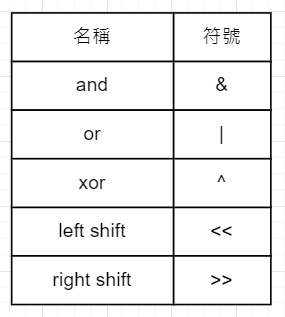
\includegraphics[scale=0.55]{images/bit_operation.png}
                \end{center}
            \end{column}
        \end{columns}
    \end{frame}
    
    \begin{frame}{位元 DP (Bitmask DP)}
        \begin{itemize}
            \item 有了位元運算之後,我們就可以將剛剛的狀態的 $x_1,x_2,\cdots,x_n$ 壓成一個數字!
            \item 假設現在 $n=4$,$x_1 = 1, x_2 = 0, x_3 = 1, x_4 = 1$
            \item 那就表示我們已經走過了 $x_1, x_3, x_4$,但還沒走過$x_2$
            \item 就可以用 $1 \times 2^3 + 1 \times 2^2 + 0 \times 2^1 + 2^0 = 13$ 表示!
            \item 所以一個狀態就可以用二進位寫成 $x_n x_{n-1} \ldots x_1$ $(x_i = 0/1)$ 
            \item 方便起見,我們會使用 0-based
        \end{itemize}
    \end{frame}
    
    \begin{frame}{位元 DP (Bitmask DP)}
        \begin{alertblock}{step 1 設置狀態}
            令 $dp[mask][i]$ 表示走過的城市為 $mask$,然後停在 $i$ 的走法數\\
            那麼答案就是 $$dp[2^n-1][n-1]$$
        \end{alertblock}
    \end{frame}

    \begin{frame}{位元 DP (Bitmask DP)}
        \setbeamercolor{block title}{use=structure,bg=green!50!black}
        \begin{block}{step 2 導出轉移}
            一個狀態若要停在 $i$,則 $mask$ 一定要走過 $i$ 這個點。而轉移可以去枚舉走過來的點 $j$
            $$dp[mask][i] := dp[mask][i] + dp[mask \oplus 2^i][j]$$
        \end{block}
    \end{frame}
    
     \begin{frame}{位元 DP (Bitmask DP)}
        \begin{block}{step 3 打好基底}
            要從第一個城市 (編號是 $0$) 開始出發,所以
            $$dp[1][0] = 1$$
        \end{block}
    \end{frame}
    
    \begin{frame}[fragile]{位元 DP (Bitmask DP)}
        \begin{lstlisting}[language=C++, basicstyle=\ttfamily\tiny]
int n,m,dp[(1<<20)][20];
vector<int> g[20];
 
void solve(){
    cin>>n>>m;
    for(int i=1;i<=m;++i){
        int u,v;cin>>u>>v;
        u--,v--;
        g[u].emplace_back(v);
    }
    dp[1][0]=1;
    for(int i=0;i<(1<<n);++i){
        for(int u=0;u<n;++u){
            if(!dp[i][u]) continue;
            if(i&(1<<u)){
                for(auto v:g[u]){
                    if(i&(1<<v)) continue;
                    dp[i^(1<<v)][v]+=dp[i][u];
                    dp[i^(1<<v)][v]%=MOD;
                }
            }
        }
    }
    cout<<dp[(1<<n)-1][n-1]<<'\n';
}
        \end{lstlisting}
    \end{frame}
    
    \begin{frame}{位元 DP (Bitmask DP)}
        \begin{block}{\href{https://cses.fi/problemset/task/1653}{CSES - Elevator Rides}}
            有 $n$ 個人和一台載重為 $x$ 的電梯,每個人的重量分別是 $w_1, \cdots, w_n$,如果要讓 $n$ 個人都搭完電梯,最少要搭幾台電梯?
            \begin{itemize}
                \item $1 \leq n \leq 20 $
            \end{itemize}
        \end{block}
    \end{frame}
    
    \begin{frame}{位元 DP (Bitmask DP)}
        \begin{itemize}
            \item 跟上一題一樣,我們可以考慮每一個人是否搭過電梯了
            \item 可是要怎麼維護要不要再搭新的電梯呢?
            \item<2-> 其實我們可以同時維護搭的電梯數跟目前電梯的重量!
        \end{itemize}
    \end{frame}
    
    \begin{frame}{位元 DP (Bitmask DP)}
        \begin{alertblock}{step 1 設置狀態}
            令 $dp[mask]$ 表示已經搭完的人為 $mask$,搭了最少電梯數跟最後一台的重量 \\
            \vspace{2.5mm}
            那麼答案就是 $$dp[2^n - 1]$$
        \end{alertblock}
    \end{frame}

    \begin{frame}{位元 DP (Bitmask DP)}
        \setbeamercolor{block title}{use=structure,bg=green!50!black}
        \begin{block}{step 2 導出轉移}
            枚舉要搭電梯的人,找到最少的答案
            $$dp[mask] = \min_{i=1}^n(dp[mask \oplus 2^i] + w[i])$$
        \end{block}
    \end{frame}
    
    \begin{frame}{位元 DP (Bitmask DP)}
        \begin{block}{step 3 打好基底}
            沒有人搭的時候,只會有一台電梯,最後一台電梯的重量為 $0$
            $$dp[0] = \{1,0\}$$
        \end{block}
    \end{frame}

    \begin{frame}[fragile]{位元 DP (Bitmask DP)}
        \begin{lstlisting}[language=C++, basicstyle=\ttfamily\tiny]
int n,x,w[20];
vector<pii> dp(1<<20);
 
void solve(){
    cin>>n>>x;
    for(int i=0;i<n;++i) cin>>w[i];
    dp[0]={1,0};
    for(int i=0;i<(1<<20);++i){
        if(i!=0) dp[i]={1e18,0};
        for(int j=0;j<n;++j){
            if(i&(1<<j)){
                pii r=dp[i^(1<<j)];
                r.S+=w[j];
                if(r.S>x) r.F++,r.S=w[j];
                dp[i]=min(dp[i],r);
            }
        }
    }
    cout<<dp[(1<<n)-1].F<<'\n';
}
        \end{lstlisting}
    \end{frame}
    
    \begin{frame}{位元 DP (Bitmask DP)}
        \begin{itemize}
            \item 注意到題目或部分分經常會有 $1 \le n \le 20$ 之類的範圍
            \item 這種時候就可以考慮嘗試位元 DP 來解決
        \end{itemize}
    \end{frame}
    
    \begin{frame}{位元 DP (Bitmask DP)}
        \begin{block}{\href{https://codeforces.com/contest/895/problem/C}{Codeforces 895C - Square Subsets}}
            給你 $n$ 個數字 $a_1, \cdots,a_n$,請問你有幾種選法可以使得選出來的數字的乘積為完全平方數。
            \begin{itemize}
                \item $1 \leq n \leq 10^5$
                \item $1 \le a_i \le 70$
            \end{itemize}
        \end{block}
    \end{frame}
    
    \begin{frame}{位元 DP (Bitmask DP)}
        \begin{itemize}
            \item 這題跟位元 dp 有甚麼關係 R
            \item<2-> 觀察 $a_i$ 的範圍!
            \item<3-> 你會發現小於 $a_i$ 的質數最多有 19 個!
        \end{itemize}
    \end{frame}
            

    \begin{frame}{位元 DP (Bitmask DP)}
        \begin{itemize}
            \item 那完全平方數有什麼特點呢? 
            \item<2-> 想想看質因數分解!
            \item<3-> 對於一個數字 $x = p_1^{\alpha_1} p_2^{\alpha_2} \cdots$ 時,所有 $\alpha_i \bmod 2$ 都是 $0$ 的話,他就是完全平方數
            \item<4-> 因此我們可以將質因數的次方的奇偶性寫成二進位的形式!
        \end{itemize}
    \end{frame}
    
    \begin{frame}{位元 DP (Bitmask DP)}
        \begin{alertblock}{step 1 設置狀態}
            令 $dp[i][mask]$ 表示用小於等於 $i$ 的數字湊出質因數分解後狀態為 $mask$ 的數量 \\
            \vspace{2.5mm}
            那麼答案就會是 $$dp[70][0]-1$$ ($-1$ 是因為不能選空的集合)
        \end{alertblock}
    \end{frame}

    \begin{frame}{位元 DP (Bitmask DP)}
        \setbeamercolor{block title}{use=structure,bg=green!50!black}
        \begin{block}{step 2 導出轉移}
            依序把 $1\sim 70$ 都加上去\\
            分成兩種情況去處理,$x[i]$ 是 $i$ 質因數分解完後的狀態
            \begin{enumerate}
                \item 加奇數個 $i$ $\Rightarrow$ $dp[i][mask] := dp[i][mask] + dp[i-1][mask \oplus x[i]]$
                \item 加偶數個 $i$ $\Rightarrow$ $dp[i][mask] := dp[i][mask] + dp[i-1][mask]$
            \end{enumerate}
            然後考慮兩種情況發生的次數
            \begin{enumerate}
                \item $C^{cnt[i]}_1 + C^{cnt[i]}_3 + \cdots$
                \item $C^{cnt[i]}_0 + C^{cnt[i]}_2 + \cdots$
            \end{enumerate}
            根據二項式定理,兩個各是 $2^{cnt[i]-1}$,可以預處理 $2$ 的次方
        \end{block}
    \end{frame}
    
    \begin{frame}{位元 DP (Bitmask DP)}
        \begin{block}{step 3 打好基底}
            空的集合的數字乘積我們預設為 $1$,最後輸出時會 $-1$
            $$dp[0][0]=1$$
        \end{block}
    \end{frame}

    \begin{frame}[fragile]{位元 DP (Bitmask DP)}
        \begin{lstlisting}[language=C++, basicstyle=\ttfamily\tiny]
int n,a[MAXN],mask[71],cnt[71],dp[2][(1<<19)];
int primes[19]={2,3,5,7,11,13,17,19,23,29,31,37,41,43,47,53,59,61,67};

int fastpow(int a,int b){
    int res=1;
    while(b){
        if(b&1) res=res*a%MOD;
        a=a*a%MOD;
        b>>=1;
    }
    return res;
} 

void pre(){
    for(int i=2;i<=70;++i){
        int now=i;
        for(int j=0;j<19;++j){
            while(now%primes[j]==0){
                now/=primes[j];
                mask[i]^=(1<<j);
            }
        }
    }
}
        \end{lstlisting}
    \end{frame}

    \begin{frame}[fragile]{位元 DP (Bitmask DP)}
        \begin{lstlisting}[language=C++, basicstyle=\ttfamily\tiny]
void solve(){
    cin>>n;
    for(int i=1;i<=n;++i){
        cin>>a[i];cnt[a[i]]++;
    }
    
    pre();
    
    dp[0][0]=1;
    for(int i=1;i<=70;++i){
        for(int j=0;j<(1<<19);++j){
            if(cnt[i]){
                dp[i%2][j]=dp[(i+1)%2][j^mask[i]]*fastpow(2,cnt[i]-1)%MOD;
                dp[i%2][j]%=MOD;
                dp[i%2][j]+=dp[(i+1)%2][j]*fastpow(2,cnt[i]-1)%MOD;
                dp[i%2][j]%=MOD;
            }else dp[i%2][j]=dp[(i+1)%2][j];
        }
    }
    cout<<(dp[0][0]-1+MOD)%MOD<<'\n';
}
        \end{lstlisting}
    \end{frame}

    \section{區間 DP (Range DP)}
    
    \begin{frame}{區間 DP (Range DP)}
        \begin{block}{\href{https://atcoder.jp/contests/dp/tasks/dp_n}{Atcoder DP Contest N - Slimes}}
            有 $n$ 個史萊姆排成一排,每次可以將相鄰的兩個大小為 $a,b$ 的史萊姆合併,並消耗 $a+b$ 的能量。請找出以最佳的方式進行合併,最少需要多少的能量。
            \begin{itemize}
                \item $1 \le n \le 400$
            \end{itemize}
        \end{block}
    \end{frame}
    
    \begin{frame}{區間 DP (Range DP)}
        \begin{itemize}
            \item 這題要怎麼做? 可以 Greedy 嗎?
            \item<2-> 我們可以來找找看反例,如果找不到你就要去證明他
            \item<3-> 來看看這個例子
        \end{itemize}
    \end{frame}
    
    \begin{frame}{區間 DP (Range DP)}
        \begin{center}
            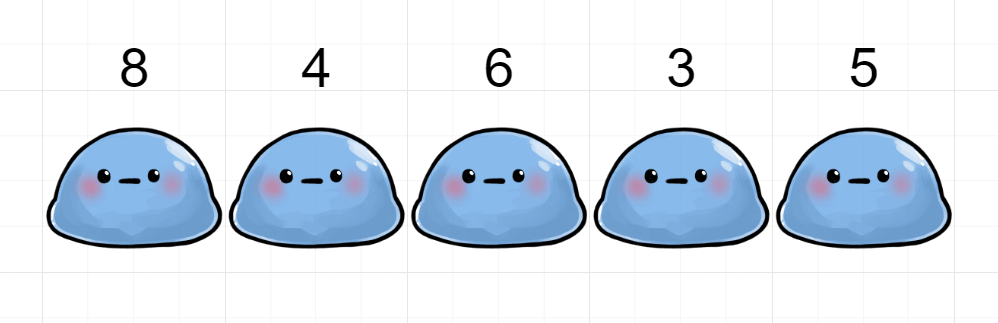
\includegraphics[width=\textwidth]{images/slimes.png}
        \end{center}
    \end{frame}
    
    \begin{frame}{區間 DP (Range DP)}
        \begin{itemize}
            \item 那我們要怎麼正確的計算答案呢?
            \item 會發現在合併的過程中,重要的只有組成兩隻史萊姆的花費及合併時的花費
            \item 因此,如果我們知道將 $[l,k]$ 和 $[k+1,r]$ 的所有史萊姆合併需要耗的最少能量
            \item 那其實我們就可以計算出 $[l,r]$ 的答案!
        \end{itemize}
    \end{frame}
    
    \begin{frame}{區間 DP (Range DP)}
        \begin{alertblock}{step 1 設置狀態}
            令 $dp[l][r]$ 表示將 $[l,r]$ 內的史萊姆合併需要的最少能量 \\
            \vspace{2.5mm}
            那麼答案就是 $$dp[1][n]$$
        \end{alertblock}
    \end{frame}
    
    \begin{frame}{區間 DP (Range DP)}
        \setbeamercolor{block title}{use=structure,bg=green!50!black}
        \begin{block}{step 2 導出轉移}
            枚舉切點 $l \le k < r$,從左右兩邊找合併後最小的答案
            $$dp[l][r] = \min (dp[l][k] + dp[k+1][r] + sum(l,r))$$
            $sum(l,r)$ 可以用前綴和在 $O(1)$ 得到
        \end{block}
    \end{frame}
    
    \begin{frame}{區間 DP (Range DP)}
        \begin{block}{step 3 打好基底}
            只有一隻史萊姆的時候,不用消耗能量
            $$dp[i][i] = 0$$
        \end{block}
    \end{frame}

    \begin{frame}[fragile]{區間 DP (Range DP)}
        Top-Down: (不用思考轉移順序,打好基底就好)
        \begin{lstlisting}[language=C++,basicstyle=\ttfamily \small]
int get(int l,int r){
    if(l==r) return 0;
    int res=1e18;
    for(int i=l;i<=r;i++)
        res=min(get(l,i)+get(i+1,r)+sum(l,r));
    return dp[l][r]=res;
}
        \end{lstlisting}
        Bottom-Up: (要注意轉移順序)
        \begin{lstlisting}[language=C++,basicstyle=\ttfamily \small]
for(int i=n;i>=1;i--){
    for(int j=i+1;j<=n;j++){
        for(int k=i;k<j;k++){
            dp[i][j]=min(dp[i][j],dp[i][k]+dp[k+1][j]+sum(i,j));
        }
    }
}
        \end{lstlisting}
    \end{frame} 
    
    \begin{frame}{區間 DP (Range DP)}
        \begin{block}{\href{https://tioj.ck.tp.edu.tw/problems/1488}{TIOJ 1488 正直 DE}}
            給你 $n$ 個矩陣,第 $i$ 個矩陣的大小為 $r_i \times c_i$。對於兩個矩陣 $A_{n \times m}$, $B_{m \times p}$ 需要的計算次數為 $nmp$。請找到將這 $n$ 個矩陣相乘所需的最少運算次數是多少?
            \begin{itemize}
                \item $1 \le n \le 1000$
            \end{itemize}
        \end{block}
    \end{frame}
    
    \begin{frame}{區間 DP (Range DP)}
        \begin{alertblock}{step 1 設置狀態}
            令 $dp[l][r]$ 表示將 $[l,r]$ 內的矩陣相乘需要的最少運算次數 \\
            \vspace{2.5mm}
            那麼答案就是 $$dp[1][n]$$
        \end{alertblock}
    \end{frame}
    
    \begin{frame}{區間 DP (Range DP)}
        \setbeamercolor{block title}{use=structure,bg=green!50!black}
        \begin{block}{step 2 導出轉移}
            枚舉切點 $l \le k < r$,從左右兩邊找合併後最小的答案
            $$dp[l][r] = \min (dp[l][k] + dp[k+1][r] + a[l] \times b[k] \times b[r])$$
        \end{block}
    \end{frame}
    
    \begin{frame}{區間 DP (Range DP)}
        \begin{block}{step 3 打好基底}
            只有一個矩陣的時候,不用任何運算次數
            $$dp[i][i] = 0$$
        \end{block}
    \end{frame}

    \begin{frame}[fragile]{區間 DP (Range DP)}
        \begin{lstlisting}[language=C++, basicstyle=\ttfamily\tiny]
signed main(){
    fastio

    int T;cin>>T;
    int sum=0;
    while(T--){
        int n;cin>>n;
        int r[n+1]{},c[n+1]{};
        for(int i=1;i<=n;++i) cin>>r[i]>>c[i];
        vector<vector<int>> dp(n+1,vector<int>(n+1,1e18));
        for(int i=1;i<=n;++i) dp[i][i]=0;
        for(int i=n;i>0;--i){
            for(int j=i;j<=n;++j){
                for(int k=i;k<j;++k){
                    dp[i][j]=min(dp[i][j],dp[i][k]+dp[k+1][j]+r[i]*c[k]*c[j]);
                }
            }
        }
        cout<<(dp[1][n]+999)/1000<<'\n';
        sum+=dp[1][n];
    }
    cout<<(sum+999)/1000<<'\n';
}
        \end{lstlisting}
    \end{frame}
    
    \begin{frame}{區間 DP (Range DP)}
        \begin{block}{\href{https://atcoder.jp/contests/dp/tasks/dp_l}{AtCoder DP Contest pL - Deque}}
            小 K 和小 B 在玩遊戲,現在有 $n$ 顆石頭排成一列。每顆石頭上面寫著一個數字 $a_i$。兩個人輪流拿石頭,每次可以拿最前面或最後面的石頭,並得到石頭上寫的數字的分數。如果兩個人都以最佳的走法 (最大化自己的分數) 去玩遊戲,兩人的分數差會是多少?
            \begin{itemize}
                \item $1 \le n \le 3000$
            \end{itemize}
        \end{block}
    \end{frame}
    
     \begin{frame}{區間 DP (Range DP)}
        \begin{itemize}
            \item 這題變成是兩個人玩遊戲欸,要怎麼處理呢?
            \item<2-> 發現到其實當先手拿完之後,後手會變成下一輪的先手
            \item<2-> 所以我們可以利用這點來設計 DP 式
        \end{itemize}
    \end{frame}
    
    \begin{frame}{區間 DP (Range DP)}
        \begin{alertblock}{step 1 設置狀態}
            令 $dp[l][r]$ 表示先手在 $[l,r]$ 內可以得到的最大分數  \\
            \vspace{2.5mm}
            那麼答案就是 $$dp[1][n]$$
        \end{alertblock}
    \end{frame}
    
    \begin{frame}{區間 DP (Range DP)}
        \setbeamercolor{block title}{use=structure,bg=green!50!black}
        \begin{block}{step 2 導出轉移}
            先手只有兩種可能性,拿最前面的石頭,或最後面的石頭
            $$dp[l][r] = \begin{cases} sum[l+1][r] - dp[l+1][r] + arr[l] &, \text{拿前面的石頭}\\ sum[l][r-1] - dp[l][r-1] + arr[r] &, \text{拿後面的石頭} \end{cases}$$
        \end{block}
    \end{frame}
    
    \begin{frame}{區間 DP (Range DP)}
        \begin{block}{step 3 打好基底}
            只有一個數字的時候,先手只能拿那個數字
            $$dp[i][i] = a[i]$$
        \end{block}
    \end{frame}
    
    \section{DP 回溯}

    \begin{frame}{DP 回溯}
        \begin{itemize}
            \item 從我們找到的最優解,往回找轉移時的路徑
            \item<2-> 乍聽之下可能會覺得不好寫,但它其實就是紀錄狀態是從哪裡轉移過來的!
        \end{itemize}
    \end{frame}
        
    \begin{frame}{DP 回溯}
        \begin{block}{\href{https://atcoder.jp/contests/dp/tasks/dp_f}{AtCoder DP Contest F - LCS}}
            給你兩個字串 $s$ 和 $t$,找出他們的 LCS
        \end{block}
        \begin{itemize}
            \item 還記得上一堂課的例題是找 LCS 的長度嗎?
            \item<2-> 但是這題要把字串回溯
        \end{itemize}
    \end{frame}

    \begin{frame}{DP 回溯}
        \begin{itemize}
            \item 現在要做的事情是紀錄狀態是從哪裡轉移過來的
            \item<2-> 令 $path[i][j] = dp[i][j]$ 這個狀態是從哪裡轉移過來的
            $$
            path[i][j]=
            \begin{cases}
                {i,j}         & \text{if } s[i]=t[j] \\
                {i+1,j}       & \text{if } dp[i+1][j] \ge dp[i][j+1]\\
                {i,j+1}       & \text{if } dp[i+1][j]<dp[i][j+1]\\
            \end{cases}
            $$
        \end{itemize}
    \end{frame}
    
    \begin{frame}[fragile]{DP 回溯}
        \begin{lstlisting}[language=C++, basicstyle=\ttfamily\tiny]
void solve(){
    string s,t;cin>>s>>t;
    int slen=s.length(),tlen=t.length();
    s=" "+s,t=" "+t;
    int dp[slen+1][tlen+1]{};
    pii r[slen+1][tlen+1]{};
    for(int i=1;i<=slen;++i){
        for(int j=1;j<=tlen;++j){
            if(s[i]==t[j]){
                dp[i][j]=dp[i-1][j-1]+1;
                r[i][j]={i-1,j-1};
            }else if(dp[i-1][j]>dp[i][j-1]){
                dp[i][j]=dp[i-1][j];
                r[i][j]={i-1,j};
            }else{
                dp[i][j]=dp[i][j-1];
                r[i][j]={i,j-1};
            }
        }
    }
    vector<char> ans;
    while(slen>0&&tlen>0){
        if(r[slen][tlen]==make_pair(slen-1,tlen-1)) ans.emplace_back(s[slen]);
        pii tmp=r[slen][tlen];
        slen=tmp.F,tlen=tmp.S;
    }
    reverse(ans.begin(),ans.end());
    for(auto i:ans) cout<<i;
}
        \end{lstlisting}
    \end{frame}
    
    \begin{frame}{DP 回溯}
        \begin{itemize}
            \item 但其實有另一種比較簡單(?)的實作方式
        \end{itemize}
    \end{frame}
    
    \begin{frame}[fragile]{DP 回溯}
        \begin{lstlisting}[language=C++, basicstyle=\ttfamily\tiny]
void solve(){
    string s,t;cin>>s>>t;
    int slen=s.length(),tlen=t.length();
    s=" "+s,t=" "+t;
    int dp[slen+1][tlen+1]{};
    for(int i=1;i<=slen;++i){
        for(int j=1;j<=tlen;++j){
            if(s[i]==t[j]) dp[i][j]=dp[i-1][j-1]+1;
            else if(dp[i-1][j]>dp[i][j-1]) dp[i][j]=dp[i-1][j];
            else dp[i][j]=dp[i][j-1];
        }
    }
    int a=slen,b=tlen,cnt=dp[slen][tlen];
    char ans[cnt+1]{};
    while(cnt>0){
        if(s[a]==t[b]){
            ans[cnt]=s[a];
            a--,b--,cnt--;
        }else if(dp[a-1][b]>dp[a][b-1]) a--;
        else b--;
    }
    for(int i=1;i<=dp[slen][tlen];++i) cout<<ans[i];
}
        \end{lstlisting}
    \end{frame}
    
    \begin{frame}{DP 回溯}
        \begin{block}{\href{https://atcoder.jp/contests/abc271/tasks/abc271_d}{AtCoder Beginner Contest 271 D - Flip and Adjust}}
            有 $n$ 張卡片,每張卡片的正面寫著 $a_i$,反面寫著 $b_i$,現在你希望可以讓這 $n$ 張卡片朝上的數字的總和為 $S$。如果存在一種作法,就輸出每張卡片要是正面還是反面。
            \begin{itemize}
                \item $1 \le n \le 10^5$
            \end{itemize}
        \end{block}
    \end{frame}

    \begin{frame}{DP 回溯}
        \begin{itemize}
            \item 不難看出這題是背包吧
            \item 而且每張卡片你要嘛選正面要嘛選反面
            \item<2-> 令 $dp[i][j][0/1] = $ 前$i$張卡片且第$i$張卡片為正面/反面時,是否能湊出$j$
            \item<3-> 紀錄每個狀態的轉移來源,就可以回朔答案了
        \end{itemize}
    \end{frame}

    % 前綴和優化
    \section{前綴和優化}

    \begin{frame}{前綴和優化}
        \begin{itemize}
            \item 當題目出現了以下這種轉移式的時候,就可以使用前綴和進行優化
            $$dp[i][j] = \sum_{k=l}^r (dp[i-1][k]) + f(i)$$
            \item 可以用 $O(n)$ 的時間預處理好前綴和,並快速地詢問答案
        \end{itemize}
    \end{frame}

    \begin{frame}{前綴和優化}
        \begin{block}{\href{https://atcoder.jp/contests/dp/tasks/dp_t}{AtCoder DP Contest pT - Permutation}}
            給你一串由 $>$ 和 $<$ 組成的字串 $s$,如果 s[i]='>' 那麼 $a_i > a_{i+1}$,反之,$a_i < a_{i+1}$。請找出總共有多少個 $1 \sim n$ 的排列滿足這個條件。 
            \begin{itemize}
                \item $1 \le n \le 3000$
            \end{itemize}
        \end{block} 
    \end{frame}
    
    \begin{frame}{前綴和優化}
        \begin{itemize}
            \item 狀態設置:令$dp[i][j] = $考慮前$i$個數字且第$j$個數字是其中第$k$大的排列數
            \item<2-> 導出轉移:
                $$\begin{cases} dp[i][j]=\sum_{k=j}^{i} dp[i-1][k] &, \text{ if } s[i] = \texttt{'>'}\\ 
                                dp[i][j]=\sum_{k=0}^{j-1} dp[i-1][k] &, \text { if } s[i] = \texttt{'<'} 
                  \end{cases}$$
            \item<3-> 打好基底: $dp[0][1] = 1$
        \end{itemize}
    \end{frame}
    
    \begin{frame}{前綴和優化}
        \begin{itemize}
            \item 轉移需要 $O(i)$ 的時間,所以總共會是 $O(n^3)$
            \item 但是其實轉移時預處理一下前綴和就可以在 $O(1)$ 的時間完成轉移
            \item 所以時間複雜度會是 $O(n^2)$
        \end{itemize}
    \end{frame}

    \begin{frame}[fragile]{前綴和優化}
        \begin{lstlisting}[language=C++, basicstyle=\ttfamily\tiny]
void solve(){
    int n;cin>>n;
    string s;cin>>s;
    s=" "+s;
    int dp[n+1][n+1]{};
    dp[1][1]=1;
    for(int i=2;i<=n;++i){
        if(s[i-1]=='>'){
            for(int j=i-1;j>=1;--j){
                dp[i][j]=dp[i][j+1]+dp[i-1][j];
                dp[i][j]%=MOD;
            }
        }else{
            for(int j=1;j<=i;++j){
                dp[i][j]=dp[i][j-1]+dp[i-1][j-1];
                dp[i][j]%=MOD;
            }
        }
    }
    int ans=0;
    for(int i=1;i<=n;++i){
        ans+=dp[n][i];
        ans%=MOD;
    }
    cout<<ans<<'\n';
}
        \end{lstlisting}
    \end{frame}
    
    \begin{frame}{前綴和優化}
        \begin{block}{\href{https://zerojudge.tw/ShowProblem?problemid=f314}{APCS 2020/10 勇者修練}}
        輸入為 $n \times m$ 大小的的陣列,每一格是一個介於 $-100$ 與 $100$ 之間的整數,表示經過這格可以累積的經驗值。你可以從最上面一排任何一個位置開始,在最下面一排任何一個位置結束。過程中每一步可以選擇往左、往右或往下走,但不能走回已經經過的位置。請你算出最多可以獲得的經驗值總和(可能是負數)。 
        \begin{itemize}
            \item $1 \le n \le 50$
            \item $1 \le m \le 10000$
        \end{itemize}
        \end{block}
    \end{frame}

    \begin{frame}{前綴和優化}
        \begin{itemize}
            \item 如果上網查詢這題的題解,你們可能會看到一個非常毒瘤的解法
            \item 查不到的我直接給你們網址 (x \href{https://sam571128.codes/2020/10/17/APCS-10-17/}{(2020 APCS 十月場)}
        \end{itemize}
    \end{frame}

    \begin{frame}{前綴和優化}
        \begin{itemize}
            \item 設 $dp[i][j]$ 表示走到 $(i,j)$ 時的最大價值
            \item 轉移式為
            $$dp[i][j] = \max \begin{cases}dp[i][k] + sum(k+1,j) &, k < j \\ dp[i][l] + sum(j,l-1) &, l > j\\ dp[i-1][j] + a[i][j]\end{cases}$$
            \item<2-> 但你會發現這個轉移式的時間複雜度為 $O(nm^2)$,顯然會 TLE
        \end{itemize}
    \end{frame}
    
    \begin{frame}{前綴和優化}
        \begin{itemize}
            \item 會發現不論是從前面開始找最大值,或是從後面找最大值
            \item 其實把這些東西存成前綴最大值跟後綴最大值一併轉移
            \item 這樣就可以在 $O(1)$ 的時間完成轉移了!
            \item 時間複雜度就變成 $O(nm)$ 了
        \end{itemize}
    \end{frame}

    % 單調隊列優化
    \section{單調隊列優化}

    \begin{frame}{單調隊列優化}
        \begin{itemize}
            \item 還記得之前講過的滑動窗口 (Sliding Window) 嗎?
            \item<2-> 我們可以用他來尋找區間極值
            \item<3-> 只要是轉移式長成這樣的時候,就可以使用
            $$dp[i] = \max_{j=1}^{k}(dp[i-j]) + f(i)$$
            \item<3-> 可以利用單調隊列優化讓轉移的複雜度變成 $O(n)$
        \end{itemize}
    \end{frame}
    
    \begin{frame}{單調隊列優化}
        \begin{block}{\href{https://zerojudge.tw/ShowProblem?problemid=c528}{Zerojudge c528. 相隔小於一定距離最小總和子序列}}
            給定一個長度為 $N$ 的整數序列 $a_1,a_2,\dots,a_N$
            及一個正整數 $K$ ,請蓋掉任意個數字使得原序列中任意的連續 $K$ 個數字都至少有一個數字被蓋掉了,請問蓋掉的數字的總和最小為多少?
            \vspace{5mm}
            \begin{itemize}
                \item $1 \le N,K \le 10^6$
            \end{itemize}
        \end{block}
    \end{frame}

    \begin{frame}{單調隊列優化}
        \begin{itemize}
            \item 如果對上一堂課熟悉,那應該可以很快的想到狀態設計和轉移
            \item<2-> 設置狀態:令 $dp[i] = $ 前 $i$ 個數字中都滿足條件而且 $a_i$ 被蓋掉了的最小總和
            \item<3-> 導出轉移:$dp[i] = \min_{j=1}^{K}(dp[i-j])+a[i]$
            \item<4-> 打好基底:$dp[0] = 0$
            \item<5-> 你會發現這個轉移式的時間複雜度是 $O(NK)$,顯然會 TLE
            \item<6-> 有發現到這個轉移式跟前一頁的很像嗎?
            \item<7-> 單調隊列優化!
        \end{itemize}
    \end{frame}

    \begin{frame}[fragile]{單調隊列優化}
        \begin{itemize}
            \item $\min_{j=1}^{K}$ 這個東西其實就是做滑動窗口最小值!
        \end{itemize}
        \begin{lstlisting}[language=C++, basicstyle=\ttfamily\small]
    deque<int> dq;
    dq.push_back(0);
    for(int i=1;i<=n;++i){
        if(!dq.empty()&&dq.front()<i-k) dq.pop_front();
        dp[i]=dp[dq.front()]+a[i];
        while(!dq.empty()&&dp[dq.back()]>=dp[i]) dq.pop_back();
        dq.push_back(i);
    }
        \end{lstlisting}
    \end{frame}
    
    \begin{frame}{單調隊列優化}
        \begin{block}{\href{https://codeforces.com/problemset/problem/372/C}{Codeforces 372C - Watching Fireworks is Fun}}
            有 $n$ 條街道,接著會放 $m$ 次煙火。第 $i$ 個煙火會有 $a_i, b_i, t_i$,表示第 $i$ 煙火會在 $t_i$ 的時間在第 $a_i$ 個街道發射,假設你在當下站在第 $x$ 個街道,會得到 $b_i-|a_i-x|$ 的快樂值。請你找到看完 $m$ 次煙火之後的最大快樂值可以是多少?
            \begin{itemize}
                \item $1\leq n\leq 150000$
                \item $1\leq m\leq 300$
            \end{itemize}
        \end{block}
    \end{frame}

    \begin{frame}{單調隊列優化}
        \begin{itemize}
            \item 我們一樣可以先列出狀態和轉移式,再去想要怎麼優化它
            \item<2-> 狀態設計:令 $dp[i][j] = $放完第 $i$ 個煙火停在座標 $j$ 的最大快樂值
            \item<3-> 導出轉移:$$dp[i][j]=\max_{k=-(t_i-t_{i-1})d}^{(t_i-t_{i-1})d}(dp[i][j],dp[i-1][j+k])+b[i]-|a[i]-j|$$
            \item<4-> 打好基底:$dp[0][j] = 0$
            \item<5-> 這個轉移式一樣是從固定大小的窗口轉移,所以可以用單調隊列優化
        \end{itemize}
    \end{frame}

    \begin{frame}[fragile]{單調隊列優化}
        \begin{lstlisting}[language=C++, basicstyle=\ttfamily\tiny]
void solve(){
    int n,m,d;cin>>n>>m>>d;
    int N=2;
    int a[m+1]{},b[m+1]{},t[m+1]{},dp[N][n+2]{};
    t[0]=1;
    for(int i=1;i<=m;++i) cin>>a[i]>>b[i]>>t[i];
    for(int i=1;i<=m;++i){
        deque<int> dq;
        for(int j=1;j<=min(n,(t[i]-t[i-1])*d+1);++j){
            while(!dq.empty()&&dp[(i+1)%2][dq.back()]<=dp[(i+1)%2][j]) dq.pop_back(); 
            dq.push_back(j);
        }
        for(int j=1;j<=n;++j){
            int sz=(t[i]-t[i-1])*d*2+1,s=j-(t[i]-t[i-1])*d,tail=j+(t[i]-t[i-1])*d;
            s=max(1LL,s),tail=min(n,tail);
            if(!dq.empty()&&dq.front()<s) dq.pop_front();
            dp[i%2][j]=dp[(i+1)%2][dq.front()]+b[i]-abs(a[i]-j);
            while(!dq.empty()&&tail+1<=n&&dp[(i+1)%2][dq.back()]<=dp[(i+1)%2][tail+1]) dq.pop_back();
            if(tail+1<=n) dq.push_back(tail+1);
            /*
            for(int k=(-t[i]+t[i-1])*d;k<=(t[i]-t[i-1])*d;++k){
                if(j+k<=n) dp[i][j]=max(dp[i][j],dp[i-1][j+k])+b[i]-abs(a[i]-j);
            }
            */
        }
    }
    int ans=-1e18;
    for(int i=1;i<=n;++i) ans=max(ans,dp[m%2][i]);
    cout<<ans<<'\n';
}
        \end{lstlisting}
    \end{frame}
    
\end{document}